\documentclass[11pt,a4paper,onecolumn]{article} 

\usepackage[brazilian]{babel}
\usepackage[utf8]{inputenc}
\usepackage{listings}
\usepackage{color}
\usepackage{xcolor}
\usepackage{fullpage}
\usepackage{indentfirst}
\usepackage{graphicx}

\title{Relatório do Capítulo 03 de\\Introdução à Programação Paralela}
\author{Lucas Sousa de Oliveira (10/59491)}
\date{\today}

\lstdefinestyle{cc}{
  belowcaptionskip=1\baselineskip,
  breaklines=true,
  frame=l,
  xleftmargin=\parindent,
  language=C,
  showstringspaces=false,
  basicstyle=\footnotesize\ttfamily,
  keywordstyle=\bfseries\color{green!40!black},
  commentstyle=\itshape\color{purple!40!black},
  identifierstyle=\color{blue!50!black},
  stringstyle=\color{orange},
  numbers=left,
  stepnumber=1,
}
\lstdefinestyle{cbash}{
  breaklines=true,
  frame=l,
  language=bash,
  basicstyle=\footnotesize\ttfamily\color{orange},
  numbers=none,
  stepnumber=1,
  rulecolor=\color{black},
  belowcaptionskip=1\baselineskip,
  xleftmargin=\parindent,
}

\begin{document}
\maketitle

\section{Título do Capítulo}
\textit{Greetings!}

\section{Objetivo}
Introduzir o aluno ao processamento paralelo e da biblioteca MPI através do estudo de um programa simples chamado \textit{\lq\lq{}Greetings!\rq\rq{}}, equivalente ao famoso \textit{\lq\lq{}Hello World!\rq\rq{}}.
\section{Resumo}
\label{sec:resumo}
No estudo de processamento paralelo, um dos componentes de maior importância é o sistema de troca de mensagens (\textit{message passing}).
Tal componente é responsável por coordenar a troca de informações entre diversos processos.
Neste capítulo utilizou-se a biblioteca MPI para tal fim.

Os programas usados neste capítulo usam o paradigma "um-programa, vários-dados" (\textit{single-program multiple-data}, SMPD).
Nesse modelo/paradigma, cada processo roda o mesmo executavel.
Entretanto, os processos executam instruções diferentes através do uso de estruturas condicionais que selecionam os processos segundo seu identificador (\textit{rank}).

O uso da biblioteca MPI requer que a diretiva
\begin{lstlisting}[style=cc,numbers=none]
#include "mpi.h"
\end{lstlisting}
seja usada para incluir os protótipos e estruturas que serão usadas.
Ainda, antes de se poder usar a biblioteca, faz-se necessário iniciá-la usando a função
\begin{lstlisting}[style=cc,numbers=none]
int MPI_Init(int* argc, char** argv[]);
\end{lstlisting}
e, simetricamente, terminá-lo usando a função
\begin{lstlisting}[style=cc,numbers=none]
int MPI_Finalize(void);
\end{lstlisting}
Outra função de grande importância é a
\begin{lstlisting}[style=cc,numbers=none]
int MPI_Comm_size(MPI_Comm comm, int* number_of_processes);
\end{lstlisting}
usada para se descobrir quantos processos foram instanciados.
Note que um comunicador é uma coleção de processos que podem enviar mensagens uns para os outros.
O comunicador padrão, predefinido, é o MPI\_COMM\_WORLD, que consiste de todos os processos em execução quando a execução do programa começa.
Um processo pode ainda descobrir seu identificador (\textit{rank}) através da função
\begin{lstlisting}[style=cc,numbers=none]
int MPI_Comm_rank(MPI_Comm comm, int* my_rank);
\end{lstlisting}

A troca de mensagens na biblioteca MPI acontece através das funções
\begin{lstlisting}[style=cc,numbers=none]
int MPI_Send(void* message, int count, MPI_Datatype datatype, int dest, int tag, MPI_Comm comm);
int MPI_Recv(void* message, int count, MPI_Datatype datatype, int source, int tag, MPI_Comm comm, MPI_Status* status);
\end{lstlisting}
onde o parâmetro \textit{message} contém a mensagem enviada/recebida, \textit{count} contém o espaço alocado para a mensagem em \textit{bytes}, \textit{datatype} possui o tipo de dados transmitidos, \textit{tag} é um identificador para diferenciar tipos de mensagens, \textit{comm} é o identificador do canal de comunicação e \textit{status} indica se a mensagem foi de fato recebida.
Existem ainda as variáveis curinga para as variáveis \textit{tag} e \textit{source}, MPI\_ANY\_SOURCE e MPI\_ANY\_TAG respectivamente, que permitem que permitem que uma chamada do MPI\_Recv receba mensagens de qualquer processo com qualquer identificador de mensagem.

O código exemplo utilizado para o desenvolvimento das atividades deste capítulo está apresentado abaixo.
\begin{lstlisting}[style=cc]
#include <stdio.h>
#include <string.h>
#include "mpi.h"

int main(int argc, char* argv[]) {
  int         my_rank;
  int         p;
  int         source;
  int         dest;
  int         tag = 0;
  char        message[100];
  MPI_Status  status;

  MPI_Init(&argc, &argv);
  MPI_Comm_rank(MPI_COMM_WORLD, &my_rank);
  MPI_Comm_size(MPI_COMM_WORLD, &p);

  if (my_rank != 0) {
    sprintf(message, "Greetings from process %d!", my_rank);
    dest = 0;
    MPI_Send(message, strlen(message)+1, MPI_CHAR, dest, tag, MPI_COMM_WORLD);
  } else {
    for (source = 1; source < p; source++) {
        MPI_Recv(message, 100, MPI_CHAR, source, tag, MPI_COMM_WORLD, &status);
        printf("%s\n", message);
    }
  }

  MPI_Finalize();
}
\end{lstlisting}

\section{Exercícios}
\subsection{Crie um arquivo contendo o programa \textit{\lq\lq{}Greetings!\rq\rq{}}. Descubra como compilar e executar em um número diferente de processadores. Qual é a saída do programa se ele for executado com apenas um processo? Quantos processadores podem ser usados?}
O comando usado para compilar um programa que utiliza a biblioteca MPI é o mostrado logo abaixo, onde \textit{code.c} é o código a ser compilado e é \textit{execultable} o executavel resultante. Tal comando usa uma instalação customizada do MPICH para gerar o executavel.
\begin{lstlisting}[style=cbash]
/opt/mpich-1.2.7/bin/mpicc code.c -o executable
\end{lstlisting}

Para rodar o executavel gerado, o comando abaixo deve ser usado. Note que \textit{nproc} deve indicar quantos processos serão iniciados e \textit{executable} indica o programa que será executado.
\begin{lstlisting}[style=cbash]
/opt/mpich-1.2.7/bin/mpirun -np nproc executable
\end{lstlisting}

Uma vez que os códigos para compilação e execução são simples, um \textit{script} pode ser criado para a simplificação destes processos. A única restrição encontrada foi o número de processos que podem ser iniciados em uma mesma máquina. Os testes realizados, apresentados na figura \ref{fig:ex1}, mostrou que apenas 254 processos podem ser executados numa mesma máquina.

\begin{figure}[h!]
  \centering
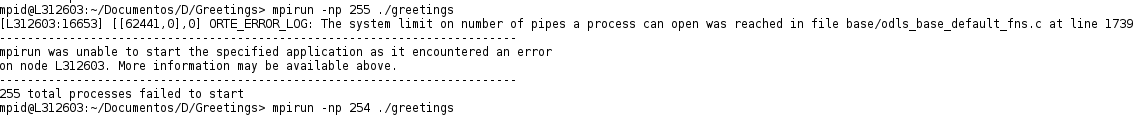
\includegraphics[width=0.98\textwidth,trim=0cm 0cm 14cm 0cm,clip=true]{../ex1/MaxProc}
  \caption{Resultado do teste para descobrir o número máximo de processos.}
  \label{fig:ex1}
\end{figure}

\subsection{Modifique o programa \textit{\lq\lq{}Greetings!\rq\rq{}} de forma que ele use elementos genéricos para \textit{source} e \textit{tag}. Existe alguma diferença na saída do programa?}
Podemos modificar o código (apresentado no final da seção \ref{sec:resumo}) da forma solicitada modificando a linha indicada abaixo. 
\begin{lstlisting}[style=cc,firstnumber=24]
MPI_Recv(message, 100, MPI_CHAR, MPI_ANY_SOURCE, MPI_ANY_TAG, MPI_COMM_WORLD, &status);
\end{lstlisting}

A diferença na saída em relação ao código original é mostrado na figura \ref{fig:ex2} a seguir. Apenas a ordem de processamento de alguns processos foi modificada.
\begin{figure}[h!]
  \centering
  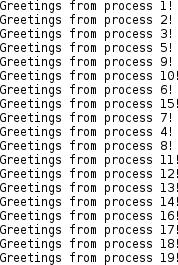
\includegraphics[]{../ex2/Resultado}
  \caption{Resultado de se modificar \textit{source} e \textit{tag} para variáveis curingas.}
  \label{fig:ex2}
\end{figure}

\subsection{Tente modificar alguns parametros de MPI\_Send e MPI\_Recv (e.g., \textit{count}, \textit{datatype}, \textit{source}, \textit{dest}). O que acontece quando se executa o programa? Ele falha? Ele pára?}
De forma a melhor analisar as modificações sugeridas, cada uma delas foi realizada individualmente.
Elas estão listadas abaixo.

\paragraph{\textit{count} no MPI\_Send} Reduzindo \textit{count} em 10 unidades observou-se lixo no resultado, possivelmente devido a remoção do caractere "\textbackslash0". Aumentar \textit{count} em 10 unidades não gerou mudanças, como esperado.
\paragraph{\textit{count} no MPI\_Recv} Apesar de se esperar o mesmo problema que no caso passado, aumentar e reduzir \textit{count} em 10 unidades não apresentou mudanças na saída.
\paragraph{\textit{datatype} no MPI\_Recv} Modificar o \textit{datatype} para MPI\_INT, MPI\_FLOAT e MPI\_BYTE não causou modificações na saída do programa. Note que tal comportamento condiz com o esperado visto que \textit{datatype} apenas altera a forma como o tamanho do \textit{buffer} de mensagem é visto. Uma vez que o tipo de dados transmitido é um caractere, representado em 8 bits, e todos os tipos disponíveis tem tamanhos maior ou igual a 8 bits, nunca seria possível observar um erro neste caso.
\paragraph{\textit{datatype} no MPI\_Send} Modificar o \textit{datatype} para MPI\_BYTE e MPI\_SHORT não causou modificações na saída do programa, mas verificou-se o erro “0 - MPI\_RECV : Message truncated” quando foi usado MPI\_INT ou MPI\_FLOAT. Note que tal erro era esperado uma vez que MPI\_INT e MPI\_FLOAT são maiores que MPI\_CHAR, fazendo com que o programa espere uma mensagem de tamanho maior. Uma vez que tal mensagem nunca chega, o erro é retornado.
\paragraph{\textit{dest} no MPI\_Send} Modificando \textit{dest} para \textit{dest}+1 faz o programa congelar. Isso acontece uma vez que o processo 0 nunca recebe as mensagens que deve imprimir, agora enviadas para o processo 1 que apenas envia mensagens.
\paragraph{\textit{source} no MPI\_Recv} Modificando \textit{source} para \textit{source}+1 faz o programa gerar o erro “0 - MPI\_RECV : Invalid rank 20”. Isso acontece porque o processo 20 não existe, visto que apenas 20 processos (do 0 ao 19) foram criados.

\subsection{Modifique o programa \textit{\lq\lq{}Greetings!\rq\rq{}} de forma que todos os processos enviam uma mensagem para o processo $\textbf{p-1}$.}
A modificação apresentada abaixo faz com que todos os processos enviem uma mensagem para o processo com um \textit{rank} imediatamente inferior.

\begin{lstlisting}[style=cc]
#include <stdio.h>
#include <string.h>
#include "mpi.h"

main(int argc, char* argv[]) {
    int         my_rank;
    int         p;
    int         source; 
    int         dest;
    int         tag = 0;   
    char        message[100]; 
    MPI_Status  status; 

    MPI_Init(&argc, &argv);
    MPI_Comm_rank(MPI_COMM_WORLD, &my_rank);
    MPI_Comm_size(MPI_COMM_WORLD, &p);

    dest = ((my_rank != 0)?(my_rank-1):p-1;
    sprintf(message, "Greetings from %d to %d!", my_rank, dest);

    MPI_Send(message, strlen(message)+1, MPI_CHAR, dest, tag, MPI_COMM_WORLD);
    MPI_Recv(message, 100, MPI_CHAR, MPI_ANY_SOURCE, tag, MPI_COMM_WORLD, &status);
    printf("%s\n",message);

    MPI_Finalize();
} 
\end{lstlisting}

\section{Trabalho de programação}
\subsection{Escreva um programa em que cada processo $\textbf{i}$ envia mensagem ao processo $\textbf{(i+1)\%p}$. (Cuidado em como $\textbf{i}$ calcula de quem deve receber a mensagem). O processo $\textbf{i}$ deverá enviar uma mensagem para $\textbf{i+1}$ e depois receber de $\textbf{i-1}$, ou o contrário? Faz diferença? O que acontece quando o programa é rodado em um processador?}

O código com as devidas modificações está mostrado abaixo. A saída do programa está na figura \ref{fig:exp}.
\begin{lstlisting}[style=cc,firstnumber=18]
#include <stdio.h>
#include <string.h>
#include "mpi.h"

main(int argc, char* argv[]) {
    int         my_rank;
    int         p;
    int         source;
    int         dest;
    int         tag = 0;
    char        message[100];
    MPI_Status  status;

    MPI_Init(&argc, &argv);
    MPI_Comm_rank(MPI_COMM_WORLD, &my_rank);
    MPI_Comm_size(MPI_COMM_WORLD, &p);

    dest = (my_rank+1)%p;

    sprintf(message, "Greetings from %d to %d!", my_rank, dest);

    MPI_Send(message, strlen(message)+1, MPI_CHAR, dest, tag, MPI_COMM_WORLD);
    MPI_Recv(message, 100, MPI_CHAR, MPI_ANY_SOURCE, tag, MPI_COMM_WORLD, &status);
    printf("%s\n",message);

    MPI_Finalize();
}
\end{lstlisting}

Note que cada processo deve primeiro enviar a mensagem para depois esperar, uma vez que se o contrário for feito, todos os processos esperarão indefinidamente uns pelos outros, o que caracteriza um \textit{deadlock}.

\begin{figure}[h!]
  \centering
  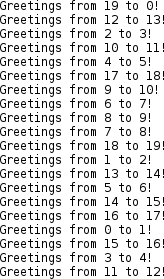
\includegraphics[]{../exp/ResultadoMod}
  \caption{Resultado do programa modificado.}
  \label{fig:exp}
\end{figure}

Quando o programa é rodado em apenas um processador espera-se que as respostas passem a ficar ordenadas, uma vez que os fatores externos que geravam o desordenamento, tais como atrasos conexão e cargas de utilização dos outros processadores, deixam de existir.

\section{Conclusão}
Conclui-se que a biblioteca MPI possui as ferramentas necessárias para o desenvolvimento de programas paralelos, inclusive com seus processos distribuidos entre várias máquinas.
Através do uso desta biblioteca pode-se construir programas segundo o modelo SPMD que trocavam informações de variadas formas.

\section{Referências}
\paragraph{Pacheco, P.S.,} (1997) \textit{Parallel Programming with MPI}. Morgan Kaufmann.

\end{document}
